\documentclass[a4paper]{article}

% Imports
\usepackage[utf8]{inputenc}
\usepackage[ngerman]{babel}
\usepackage[T1]{fontenc}
\usepackage{fancyhdr}
\usepackage{caption}
\usepackage{float}
\usepackage{subcaption}
\usepackage{epigraph}
\usepackage[acronym]{glossaries}
\usepackage{graphicx}
\usepackage{tabularx}
\usepackage{cite}
\usepackage{hyperref}

% Generate the glossary
\makeglossaries

% Title page
\title{Open Source Software \\
    \noindent\rule[0.25ex]{\linewidth}{0.5pt}
    \large Wie nehmen Endanwender Open Source Software wahr?
}

\author{
  Blechschmidt, Til\\
  \texttt{til@blechschmidt.de}\\
  Nordakademie, Elmshorn
  \and
  Peeters, Noah\\
  \texttt{noah.peeters@icloud.com}\\
  Nordakademie, Elmshorn
}

% Numbering
\setcounter{secnumdepth}{3}
\setcounter{tocdepth}{2}

% Quote styling
\setlength\epigraphwidth{.8\textwidth}
\setlength\epigraphrule{0pt}

% Glossary
\newacronym{oss}{OSS}{Open Source Software}
\newglossaryentry{css}{name={Closed Source Software}, description={Software, deren Source Code im Gegensatz zu \gls{oss} nicht offen für jeden einsichtig hat.}}

\begin{document}
    % Title page
    \thispagestyle{fancy}
    \maketitle

    % Abstract
    \clearpage
    \begin{abstract}
         \gls{oss} wird in vielen Bereichen von Betriebssystemen über Anwendersoftware bis hin zu kommerziellen Produkten eingesetzt. Es gibt bereits Studien zu dem Einsatz von quelloffener Software aus der Sicht von kommerziellen Betrieben. Gegenstand dieser Arbeit ist es die Situation aus der Perspektive der Endanwender darzulegen und mit der der Unternehmen zu vergleichen.
    \end{abstract}
    \newpage

    % TOC
    \tableofcontents
    \listoffigures
    \listoftables
    \clearpage

    % --- Content ---
    
    \glsresetall                
    \section{Fragestellung}\label{section:fragestellung}
        In der Arbeit soll die Frage, inwiefern Endanwender Open Source Software wahrnehmen, untersucht werden. Dabei soll nicht nur die \emph{direkte} Verwendung von \gls{oss}, wie es zum Beispiel bei LibreOffice der Fall ist, eine Rolle spielen, sondern auch die \emph{indirekte} Nutzung als Komponente kommerzieller Lösungen wie Chromium als Grundbaustein von Google Chrome\footnote{Genaue Definitionen sind in \ref{section:indirekte_nutzung} zu finden.}.
		
		Es wird erwartet, dass viele Nutzer unbewusst und indirekt mit \gls{oss} in Kontakt stehen, sie diese also als Teil größerer, kommerzieller \gls{css} nutzen, sich dessen aber nicht bewusst sind. Außerdem ist zu erwarten, dass nur ein kleiner Teil der Anwender direkt mit \gls{oss} interagiert\cite{oss:lotus-to-linux}. Ausserdem ist zu erwarten, dass Nutzer mit höheren Computerkenntnissen mehr über \gls{oss} wissen.

		\subsection{Definitionen} % TODO: Achtung Reihenfolge Definitionen/Fragestellung
            \subsubsection{\acrlong{oss}}
                \begin{quote} 
                    \centering 
                    Software wird als Open Source bezeichnet, wenn ihr Quelltext frei zugänglich ist. Sie kann in kommerzieller Software eingesetzt werden, ihre Nutzung muss allerdings nicht kostenfrei sein. 
                \end{quote}
                
            \subsubsection{Nutzung von \acrlong{oss}}\label{section:indirekte_nutzung}
                Die Nutzung von Open Source Software durch Endanwender kann in zwei Arten unterteilt werden.
                
                \paragraph{Direkte Nutzung}
                    Zum einen gibt es die direkte Nutzung, bei der der Nutzer eine Software verwendet, die Open Source ist, also dessen Source Code frei zugänglich ist.
                    
                    Beispiele für Direkte Nutzung:
                    \begin{itemize}
                        \item Wikipedia
                        \item Thunderbird % TODO: mehr Beispiele
                    \end{itemize}
                    
                \paragraph{Indirekte Nutzung}
                    Zum anderen gibt es die indirekte Nutzung. Hier verwendet der Nutzer Software, dessen Source Code nicht frei zugänglich ist, deren Funktionalität aber entscheidend von \gls{oss} Komponenten abhängt. Ohne diese Komponenten wäre die Funktionalität stark eingeschränkt. Hierbei werden folgende Komponenten \textbf{nicht} berücksichtigt:
                    
                    \begin{itemize}
                        \item Entwicklerwerkzeuge wie Compiler
                        \item Datenbanken wie MySQL
                        \item Betriebssysteme wie Linux 
                    \end{itemize} % TODO: gibt es mehr? Apache Web server?
                    Der Grund dafür liegt in der Verbreitung dieser Komponenten. % TODO: bessere Erklärung
                    
                    Beispiele für Indirekte Nutzung:
                    \begin{itemize}
                        \item Google Chrome % TODO add reference to table
                        \item macOS % TODO add reference to table
                    \end{itemize}
                    % TODO: mehr Beispiele

            
        
    \section{Design und Durchführung}
        Um zuverlässige Daten zu erhalten, die die aktuelle Wahrnehmung der Endanwender widerspiegeln, wurde eine Umfrage durchgeführt. Für die Sicherstellung der Repräsentativität der Umfrage wurden mindestens 80 Antworten erwartet.\label{section:fragestellung:answerAmount}
		Die Umfrage wurde überwiegend quantitativ mit geschlossenen Fragen gestaltet, um den Aufwand für die Befragten zu minimieren und damit die Teilnehmerrate und Datenmenge zu maximieren.  % TODO: Cite
    
		Zweck der Befragung ist es, einen repräsentativen Überblick über die Wahrnehmung von Open Source Software des Endanwenders zu erhalten. Dabei soll Aufschluss über die Verteilung von indirekter und direkter Nutzung gegeben werden. Außerdem soll evaluiert werden, welche Gründe die Nutzer für und gegen die Nutzung von Open Source Software sehen. % TODO: genauer mit der Umfrage abgleichen
	
		\subsection{Design}
		  \subsubsection{Aufbau}
    			Die Erhebung ist in vier Teile gegliedert, die im Folgenden näher erläutert sind: 
    		   
    			\paragraph{Bewusste Nutzung}
    				Um die, dem Anwender bewusste, Nutzung von Open Source Software zu erheben, beginnt die Umfrage mit diesem Abschnitt.\\
    				Zunächst wird ermittelt, ob die Nutzer wissen, was Open Source Software ist. Um im weiteren Verlauf der Umfrage sinnvolle Antworten zu erhalten, wird anschließend die Definition von Software sowie quelloffener Software erklärt.\\
    				Nun werden Fragen zum Nutzungsverhalten von solcher Software gestellt ohne dabei Beispiele zu nennen, um Beeinflussung zu vermeiden.
    			
    			\paragraph{Unbewusste Nutzung}
    				Im zweiten Abschnitt werden konkrete Beispiele für Open Source Software genannt, um die Nutzer darauf aufmerksam zu machen, wo Open Source Komponenten und Softwares überall eingesetzt werden, ohne dass es ihnen klar ist.\\
    				Außerdem soll geklärt werden, warum es Differenzen, wenn vorhanden, zwischen bewusster und unbewusster Nutzung gibt.
    			
    			\paragraph{Gründe für und gegen Open Source Software}
    				Im dritten Abschnitt werden Fragen bezüglich der Nutzungs- und Hinderungsgründe von Open Source Software gestellt. Dazu wird gefragt, warum oder warum nicht Endnutzer oder Unternehmen Open Source Software einsetzten. Die möglichen Antworten werden aus der Schweizer Studie zum Thema Open Source\cite{oss:studie} genommen, um die Wahrnehmung mit der realen Nutzung vergleichbar zu machen.
    			
    			\paragraph{Demographische Differenzen}
    				Zur Analyse von Differenzen innerhalb der Bevölkerungen enthält die Umfrage Fragen zur aktuellen Tätigkeit\footnote{Schüler, Student, Arbeitnehmer, etc.} sowie zur Selbsteinschätzung der Computerkenntnisse.
				
			\subsubsection{Designentscheidungen}
			 \begin{itemize}
			     \item Es wurde überwiegend auf Freifelder verzichtet, um die Auswertung zu vereinfachen. Aus dem selben Grund wurde bei dem eingesetzten Freifeld ein einheitliches Format gefordert.
				\item Bei Skalen wurde darauf geachtet eine gerade Anzahl an Optionen anzubieten, um den Nutzer nicht die Möglichkeit zu bieten neutral zu antworten.
				\item Die Texte sollen möglichst allgemeinverständlich geschrieben sein, um auch Nutzern ohne technischen Hintergrund die Teilnahme an der Umfrage zu ermöglichen.
			 \end{itemize}
			 
			 \subsubsection{Softwarebeispiele}
			     \begin{table}[!htbp]
			         \centering
			         \begin{tabularx}{\textwidth}{rcX}
			               Name & OSS & Quelle\\\hline\hline
			               Firefox & Ja & \tiny\url{https://www.openhub.net/p/firefox} [Online; letzter Zugriff 06.03.1018] \\
			               Chrome & Ja & \tiny\url{https://www.chromium.org} [Online; letzter Zugriff 26.02.1018] \\
			               Safari & Ja & \tiny\url{https://developer.apple.com/opensource/} [Online; letzter Zugriff 26.02.1018]\\
			               Chromium & Ja & \tiny\url{https://www.chromium.org} [Online; letzter Zugriff 26.02.1018] \\
			               Opera & Ja & \tiny\url{https://dev.opera.com/blog/300-million-users-and-move-to-webkit/}\\\hline
			               Windows & Nein & \tiny\url{https://www.microsoft.com/en-us/windows/get-windows-10} [Online; letzter Zugriff 06.03.1018]\\
			               macOS & Nein & \tiny\url{https://developer.apple.com/opensource/} [Online; letzter Zugriff 26.02.1018] \\
			               Linux & Ja & \tiny\url{https://www.kernel.org/category/faq.html} [Online; letzter Zugriff 06.03.1018] \\
			               Android & Ja & \tiny\url{https://source.android.com} [Online; letzter Zugriff 06.03.1018] \\
			               iOS & Nein & \tiny\url{https://developer.apple.com/opensource/} [Online; letzter Zugriff 26.02.1018] \\\hline
			               Wikipedia & Ja & \tiny\url{https://www.mediawiki.org/wiki/Download} [Online; letzter Zugriff 26.02.1018]\\
			               Moodle & Ja & \tiny\url{https://docs.moodle.org/dev/Main_Page} [Online; letzter Zugriff 06.03.1018] \\
			               ownCloud/NextCloud & Ja & \tiny\url{https://owncloud.org/faq/} [Online; letzter Zugriff 06.03.1018] \\\hline
			               Open-/LibreOffice & Ja & \tiny\url{https://openoffice.apache.org/get-involved.html} [Online; letzter Zugriff 06.03.1018] \\
			               Microsoft Office & Nein & \tiny\url{https://products.office.com/en-US/} [Online; letzter Zugriff 06.03.1018]\\
			               LaTeX & Ja & \tiny\url{https://www.tug.org/texlive/svn/} [Online; letzter Zugriff 06.03.1018] \\
			               GIMP & Ja & \tiny\url{https://www.gimp.org/about/} [Online; letzter Zugriff 06.03.1018]\\
			               Photoshop & Nein & \tiny\url{https://www.photoshop.com} [Online; letzter Zugriff 06.03.1018]\\
			               VLC & Ja & \tiny\url{https://www.videolan.org/vlc/download-sources.html} [Online; letzter Zugriff 06.03.1018]\\
			               Windows Media Player & Nein & \tiny\url{https://support.microsoft.com/en-us/help/14209} [Online; letzter Zugriff 06.03.1018]\\
			               Thunderbird & Ja & \tiny\url{https://support.mozilla.org/en-US/kb/thunderbird-faq} [Online; letzter Zugriff 26.02.1018] \\
			               7-Zip & Ja & \tiny\url{http://7-zip.org} [Online; letzter Zugriff 06.03.1018]\\
			               WinRAR & Nein & \tiny\url{https://www.rarlab.com} [Online; letzter Zugriff 06.03.1018]
			         \end{tabularx}
			         \caption{Liste mit Software, die in der Umfrage verwendet wurde}
			         \label{table:software_examples}
			     \end{table}
			     
		\subsection{Durchführung}
            \subsubsection{Software}
                Die Umfrage wurde mithilfe von Google Forms\footnote{\url{https://www.google.com/forms/about/}} erstellt und durchgeführt. Anschließend wurden die Daten als CSV exportiert, mithilfe von Swift\footnote{\url{https://swift.org/about/}} strukturiert und unter Zuhilfenahme von Numbers\footnote{\url{https://www.apple.com/numbers/}} grafisch dargestellt. Sämtliche Swift-Programme die zur Strukturierung verwendet wurden sind open-source auf GitHub\footnote{\url{https://github.com/TexNAK/OpenSource/tree/master/src/Auswertung}}.
            \subsubsection{Verbreitung}
                Um die Reichweite der Umfrage zu maximieren und die Kosten zu minimieren wurde diese in Form einer Onlinebefragung umgesetzt. Dabei wurden Kanäle wie Social Media, E-Mail, Messenger genutzt, um auf die Umfrage aufmerksam zu machen. Zudem wurde der Link zu der Umfrage über private Kontakte und an der Nordakademie verbreitet.
                
    \section{Auswertung}
        \subsection{Vorgehen}\label{section:auswertung:vorgehen}
            \paragraph{Auswertung des Freifeldes}
                Um mit den Daten des Freifeldes zu arbeiten, wurden zunächst alle Begriffe, die die Nutzer eingegeben haben, einer Kategorie zugeordnet. Alle Begriffe, denen kein sinnvoller Inhalt zugeordnet werden konnte, wurden in der Kategorie '-' zusammengefasst. Diese Zuordnung ist in Tabelle \ref{table:categories} dargestellt.\\

            
            \begin{table}[!htbp]
                \begin{tabularx}{\textwidth}{rX}
                    Kategorie & Begriffe (Lower case) \\
                    \hline
                    - & \tiny geht, ?, hilfee, komische, privat, , !, nutze, wissentlich, nix, ibt, immer noch nicht verstanden was es ist, weil, keine ahnung, .., ich, blub, frage, tue, meist ohne opensource, benutze, modell, ..., warum ist das hier pflichtfeld?, bla, es sie g, nicht, ohne, und, ich nicht\\
                    Alternativlos & \tiny alternativlos, keine alternative\\
                    Anpassbarkeit & \tiny vielfältigkeit, man kann selber eingreifen, teilweise anbassbar, zeitvertreib, benutzerindividuell, vielseitig, offen für eigene entwicklungen, anpassbarkeit, erweiterbar, kontrolle, flexible, individuell, kompatibler, erweiterungen, anpassbar, variantenreich\\
                    Auswahl & \tiny auswahl\\
                    Benutzerfreundlichkeit & \tiny sympathisch, verwaltung, schön, einfach, moderrn, freundlich zu bedienen, handhabbar, anwendungsnutzen, verständlich\\
                    Code Veränderbarkeit & \tiny änderbar, veränderbar, offener quelltext\\
                    Community & \tiny jeder kann mitmachen, community, große community, wurde empfohlen, demokratisch, communitysupport, guter support/foren, verbreitet, communitydriven, großer nutzenkreis, anleitungen, community"", sozial, viel hilfestellung im internet, oft verbreitet\\
                    Datenschutz & \tiny vertrauenswürdigkeit, datenschutz, privatsphäre, datensicherheitt\\
                    Entwickler Community & \tiny mit pacman installierbar, updatefrequenz, schnellere sofwareentwicklung, große entwickler gemeinschaft\\
                    Erfahrung & \tiny erprobt, erfahrung, gewohnheit\\
                    Frei & \tiny offene standards, freiheit, verifizierbar, keine geheimnisse, quellcode, open standard, frei, openess, freiheit (fsf)\\
                    Funktionalität & \tiny teilweise mehr funktionen als normale programme, weils funktioniert, funktionalität, funktionsbereitstellung\\
                    Grundeinstellung & \tiny gutes gefühl, prinzip, open source unterstützen, moralischer, überzeugung, weltanschauung, moral, philosophie\\
                    Hilfreich & \tiny hilfreich\\
                    Indirekte Nutzung & \tiny fast überall ist oss enthalten\\
                    Innovation & \tiny innovativ, kreativ, gutes konzept, innovation\\
                    Kompatibilität & \tiny kompatibel, kompatibilität\\
                    Kosten & \tiny free, teilweisekostenfrei, kostenvorteil, kostenlos, gratis, billig, kostengünstig, günstig, kostenersparnis, kosten, umsonst, preis, preiswert, oft kostenlos, for free, kostenfrei, häufig kostenlos, meistens kostenlos, meist kostenlos\\
                    Notwendig & \tiny arbeit, notwendigkeit, abeit\\
                    Nützlich & \tiny praktisch, nützlich\\
                    Qualität & \tiny teilw. besser, oft gute alternative, besser als kommerzielle sw, besser, gute alternative, gut, stabilität, plattformunabhängig, ""schlechter"" als nicht open source, meistens aktuell, funktioniert, aktuell, zuverlässig, zielorientierung, qualität, schnell, stable, fast genauso wie vergleichbare programme, oft besser, manchmal besser, toll, fehlerfreiheit\\
                    Sicherheit & \tiny ""sicher, sicher, sicherheit, sicherer\\
                    Testversion & \tiny testversion\\
                    Transparenz & \tiny transparent, transparant, transparenz, offen\\
                    Unabhängigkeit & \tiny unabhängigkeit, keine großen konzerne unterstützen, against microsoft, unabhängig von herstellern, anti-kommerz, unabhängig\\
                    Unbewusste Nutzung & \tiny unbewusst\\
                    Verfügbarkeit & \tiny schneller zugriff, einfach zu bekommen, verfügbarkeit, freizugänglich, leicht zugänglich, schnell verfügbar als download, gut zugänglich, verfügbar\\
                    Vertrauen & \tiny vertrauen\\
                    Weiterentwicklung & \tiny weiterentwicklung\\
                    Zufall & \tiny keine gründe, hat keinen speziellen grund, zufall, weil software die ich brauche zufällig open-source ist\\
                \end{tabularx}
                \caption{Zuordnung: Begriffe des Freifeldes zu Kategorien}
                \label{table:categories}
            \end{table}
            
            Im späteren Verlauf der Arbeit werden die Werte des Freifelds mit den Ergebnissen einer Schweizer Studie verglichen. Dazu bedarf es einer Zuordnung zu den vorliegenden Kategorien aus der Studie, welche in Tabelle \ref{table:privateToCommercialCategories} dargelegt ist.\\
            
            \begin{table}
                \centering
                \bgroup
                \def\arraystretch{1.5}
                \begin{tabular}{ r | l }
                    Freifeld Kategorie & Schweizer Studie\\ \hline
                    Kosten & Kosteneinsparungen\\
                    Anpassbarkeit & Anpassbarkeit\\
                    Unabhängigkeit & Unabhängigkeit\\
                    Grundeinstellung & Offene Standards\\
                    Transparenz & Transparenz\\
                    Community & Community\\
                    Innovation & Innovation\\
                    Sicherheit & Sicherheit\\
                    Weiterentwicklung & Mitarbeitende\\
                    Qualität & Stabilität
                \end{tabular}
                \egroup
                \caption{Zuordnung: Freifeld Kategorien zu Aspekten der Schweizer Studie}
                \label{table:privateToCommercialCategories}
            \end{table}
            
            \paragraph{Auswertung der Anwendungsmatrix}
                Bei der Auswertung der Anwendungsmatrix wird in der gesamten Arbeit immer nur auf die Antworten der Nutzer eingegangen, die auch angaben die Software zu nutzen. Die Gründe hierfür werden in Abschnitt \ref{section:selbstreflexion} Selbstreflexion beleuchtet.
                %TODO: Nur wenn man die Software nutzt -> ref zu selbstreflexion
            
        \subsection{Validität der Ergebnisse}
            Der Eingangs auf Seite \pageref{section:fragestellung:answerAmount} erwähnte Umfang von 80 Antworten wurde mit 119 Datensätzen zum Zeitpunkt der Auswertung übertroffen. Die Stichprobe ist somit groß genug um signifikante Schlussfolgerungen im Bezug auf die Leitfrage zu ziehen. % TODO Give reason why
            \subsubsection{Demographische Gruppen}\label{section:demographic_groups}
                Abbildung \ref{fig:rowsPer:activity} legt dar, dass der Anteil der Schüler nur sehr gering ist und diese Gruppe mit nur acht Teilnehmern nicht repräsentativ ist. Des Weiteren ist zu beachten, dass der Anteil von Personen mit sehr hohen (6) und hohen (5) Computerkenntnissen nach Abbildung \ref{fig:rowsPer:knowledge} einen Großteil der Befragten ausmacht. In Abbildung \ref{fig:rowsPer:knowledgeCite} sind die Werte einer unabhängigen Studie der Österreichischen Computer Gesellschaft\cite{demographicDistributionKnowledge} dargestellt, welche eine weitreichende Übereinstimmung mit der Verteilung der Stichprobe dieser Arbeit haben. Folglich können repräsentative Aussagen im Bezug auf den Kenntnisstand der Nutzer getätigt werden.
            
        \begin{figure}[h]
            \centering
            \begin{minipage}{.5\textwidth}
                \centering
                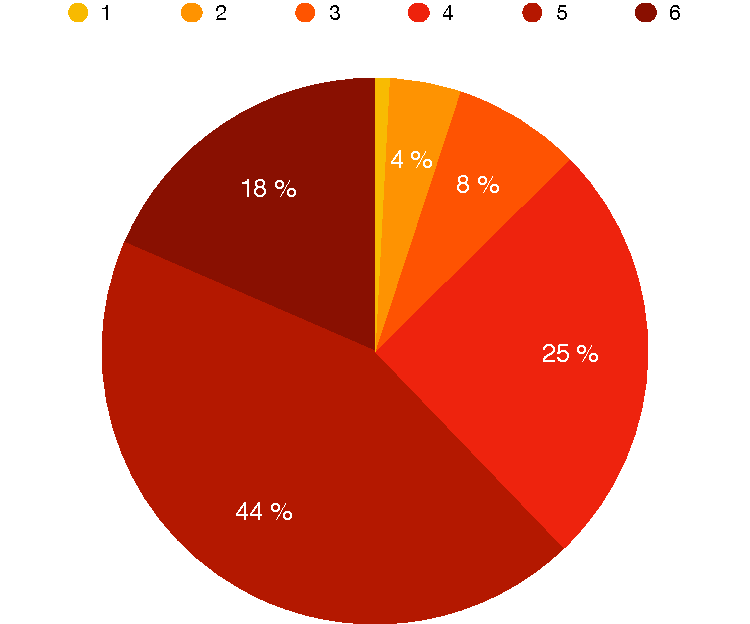
\includegraphics[width=\textwidth]{assets/results/validity/rowsPerKnowledge}
                \subcaption{Kenntnisstand}
                \label{fig:rowsPer:knowledge}
            \end{minipage}%
            \begin{minipage}{.5\textwidth}
                \centering
                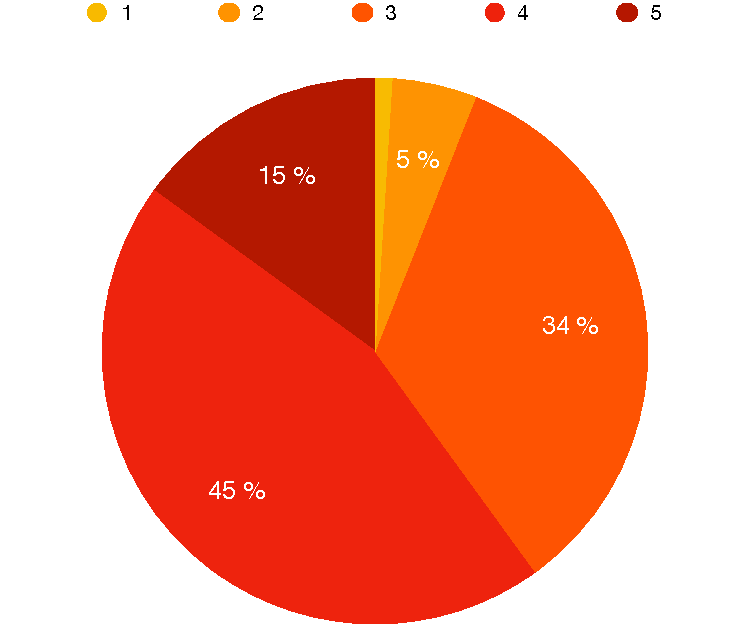
\includegraphics[width=\textwidth]{assets/results/validity/knowledgeComparisonCite}
                \subcaption{Kenntnisstand | Vergleichsstudie}
                \label{fig:rowsPer:knowledgeCite}
            \end{minipage}
            
            \centering
            \begin{minipage}{.5\textwidth}
                \centering
                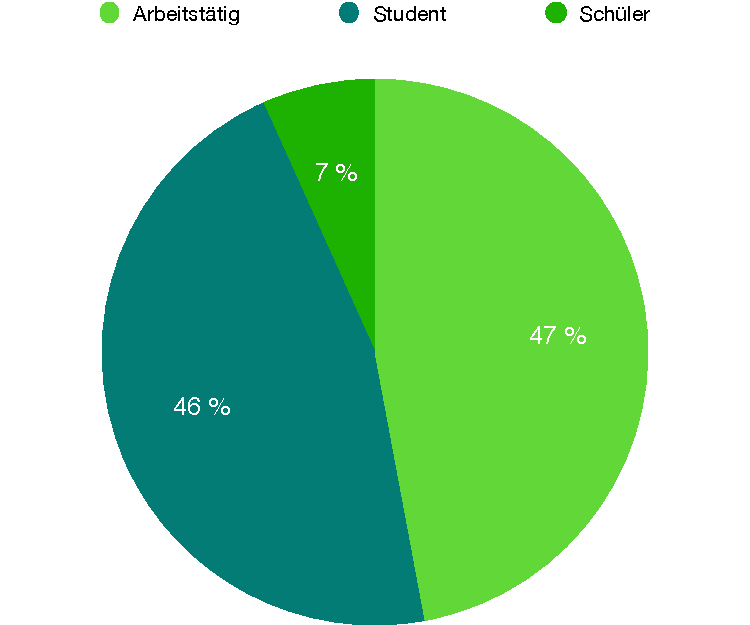
\includegraphics[width=\textwidth]{assets/results/validity/rowsPerActivity}
                \subcaption{Beschäftigung}
                \label{fig:rowsPer:activity}
            \end{minipage}
            \caption{Anteile der Stimmen}
        \end{figure}

    \section{Ergebnisse}
        %TODO: Einleitung 3 Aspekte etc.
        \subsection{Wissen über OSS}\label{section:knowledge_oss}
            Ein entscheidender Aspekt der Wahrnehmung von \gls{oss} durch Endnutzern ist, ob diese wissen, ob es sich bei Software um \gls{oss} handelt oder diese \gls{oss} verwendet.
            
            % TODO reference zu kritik: Nur daten, wenn oss genutzt
            Um dies zu ermitteln, wurde im Abschnitt \emph{Nutzungsverhalten} der Umfrage gefragt, welche Anwendungen aus einer vorgegebenen Liste\footnote{Siehe Tabelle \ref{table:software_examples}} genutzt werden und welche Open Source sind oder \gls{oss} nutzt. Die Daten wurden mit Hilfe von Abbildung \ref{figure:knowledge_difference} ausgewertet.
            
                        
            \begin{figure}
                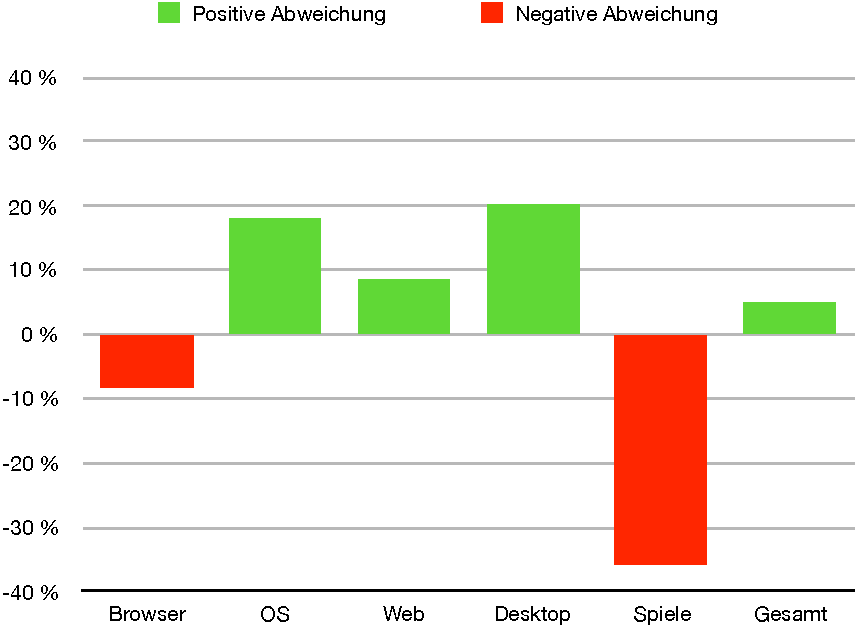
\includegraphics[width=\textwidth]{assets/results/openSourceJudging/openSourceJudgingDetailedOSSOnly2.pdf}
                \caption{Abweichung des Wissens über \gls{oss} von $50 \%$.}
                \label{figure:knowledge_difference}
            \end{figure}
            
            
            \subsubsection{Aufbau des Diagramms}
                \paragraph{Kategorien}
                    Für die Auswertung wurden die Anwendungen wie auch schon bei der Umfrage in die Kategorien Browser, Betriebssysteme (OS), Web und Desktop gruppiert.
                    
                \paragraph{Werte}
                    Zunächst ist zu betrachten, wie das Ergebnis ausfallen würde, wenn alle Befragten raten würden. In diesem Fall wäre der Erwartungswert die Hälfte der Befragten, da es sich um eine Ja-Nein-Frage, also eine Frage mit nur zwei Möglichkeiten, handelt
                    
                    Um also die Ausgangsfrage bewerten zu können ist es notwendig sich die Differenz zwischen $50\%$\footnote{In der Umfrage war diese Frage als `Checkbox` umgesetzt, die den Standardwert \emph{Nein} hat. Wie in Abschnitt \ref{section:selbstreflexion} beschrieben kann es hierdurch zu einer Senkung des Erwartungswertes kommen. Hier wird dennoch mit 50\% gerechnet, um eine Auswertung möglich zu machen.}. und dem Ergebnis der Umfrage zu betrachten. Dabei kann es zu drei möglichen Fällen kommen:\\
            
                    \begin{tabularx}{\textwidth}{rX}
                        \textbf{Ergebnis} & \textbf{Auswertung} \\\hline
                        $= 50 \%$ & Die Befragten haben haben das selbe Ergebnis erreicht, wie beim Raten. Das bedeutet, dass im Durchschnitt kein Wissen über \gls{oss} vorhanden ist.\\
                        $> 50 \%$ & Ein größerer Teil der Befragten konnten die Frage richtig beantworten. Das bedeutet, dass im Durchschnitt richtiges Wissen über \gls{oss} vorhanden ist. Im Extremfall 100\% konnte jeder der Befragten die Frage richtig beantworten.\\
                        $< 50 \%$ & Ein größerer Teil der Befragten hat die Frage falsch beantwortet. Das bedeutet, dass im Durchschnitt falsches Wissen über \gls{oss} vorhanden ist. Im Extremfall 0\% hat keiner der Befragten die Frage richtig beantworten.  
                    \end{tabularx}
            
                \paragraph{Auswahl der Datenpunkte}
                    Wie in Abschnitt \ref{section:auswertung:vorgehen} erläutert wurden bei der Auswertung nur die Antworten von Nutzern in die Auswertung einbezogen, die auch angegeben haben die Software zu verwendet.
                                        
            \subsubsection{Auswertung des Diagramms}\label{section:knowledge_analysis}
                In dem Graphen wird deutlich, dass das Wissen über \gls{oss} stark von der Kategorie abhängig ist. %TODO: add more content
            
                Nimmt man an, dass $r \in \left[0...1\right]$ Prozent der Befragten sicher wussten, dass es sich um \gls{oss} Software handelt, bedeutet dies, dass $d = 1 - r$ Prozent geraten haben. Unter Einbezug des Erwartungswertes von $50 \%$ beim Raten erhält man dann als Gesamt-Erwartungswert $\mu$:
            
                \begin{equation}
                \begin{split}
                    \mu &= r + \frac{d}{2} \\
                        &= \frac{2r + 1 - r}{2} \\
                        &= \frac{r + 1}{2} \\
                    r   &= 2\mu - 1
                \end{split}
                \end{equation}
            
                Mit dieser so erhaltenen Formel für $r$ lässt sich der reale Anteil der Befragten ermittelt, die in der Lage waren richtig zu beantworten, ob es sich bei einer Anwendung um \gls{oss} handelt oder sie diese nutzt. Die sich daraus ergebenen Werte für den realen Prozentanteil sind in Tabelle \ref{table:knowledge_by_category} dargestellt. Negative Werte bedeuten dabei wie auch in der vorangegangenen Abbildung \ref{figure:knowledge_difference}, dass falsches Wissen vorhanden ist.
                
                %TODO: Auswertung
                
                \begin{table}
                    \centering
                    \begin{tabular}{rcccc}
                        Kategorie & Umfang & Erfolge & Prozent Statistik & Prozent Realität \\\hline\hline
                        Browser & $246$ & $103$ & $41.87\%$ & $-16.26\%$\\
                        OS & $122$ & $83$ & $68.03\%$ & $36.07\%$\\
                        Web & $181$ & $106$ & $58.56\%$ & $17.13\%$\\
                        Desktop & $278$ & $195$ & $70.14\%$ & $40.29\%$\\\hline
                        Gesamt & $827$ & $487$ & $58.89\%$ & $17.78\%$
                    \end{tabular}
                    \caption{Wissen über \gls{oss} nach Kategorien}
                    \label{table:knowledge_by_category}
                \end{table}
                
                \paragraph{Positive Abweichung}
                    Besonders gut haben Desktop Anwendungen ({\scriptsize 40.29\%}) und Betriebsysteme ({\scriptsize 36.07\%}) abgeschnitten.
                    
                    Bei Betriebssystemen lässt sich dieses gute Ergebnis damit erklären, dass Linux häufig als Beispiel für \gls{oss} verwendet wird und damit auch andere Desktop Betriebssysteme als nicht \gls{oss}.%TODO: Citation needed.
                    %TODO: Hier Auswertung vervollständigen.
                    
                    %TODO: Desktop
                
                \paragraph{Negative Abweichung}
                    Bei Browsern scheint nicht bekannt zu sein, dass sowohl Apple mit WebKit als auch Google mit Chromium den Kern ihrer Browser als \gls{oss} veröffentlicht haben\footnote{Siehe Tabelle \ref{table:software_examples}}, da hier falsches Wissen ({\scriptsize -16.26\%}) vorhanden ist.                        %TODO: Wie sieht es mit den oss Browsern aus. Hier Auswertung vervollständigen. 
                    
                \paragraph{Signifikanz der Abweichung}
                
                \begin{table}
                    \centering
                    \begin{tabular}{rccccc}
                        Kategorie & Umfang & Erfolge & $2\sigma$-Umgebung & $3\sigma$-Umgebung & Signifikanz \\\hline\hline
                        Browser & $246$ & $103$ & \tiny [ 107.3156 ; 138.6844 ] & \tiny [ 99.4734 ; 146.5266 ] & Signifikant\\
                        OS & $122$ & $83$ & \tiny [ 49.9546 ; 72.0454 ] &  \tiny [ 44.432 ; 77.568 ] & Hoch\\
                        Web & $181$ & $106$ & \tiny [ 77.0464 ; 103.9536 ] &  \tiny [ 70.3196 ; 110.6804 ] &  Signifikant\\
                        Desktop & $278$ & $195$ & \tiny [ 122.3267 ; 155.6733 ] & \tiny [ 113.99 ; 164.01 ] & Hoch\\\hline
                        Gesamt & $827$ & $487$ & \tiny [ 384.7424 ; 442.2576 ] & \tiny [ 370.3636 ; 456.6364 ] & Hoch
                    \end{tabular}
                    \caption{Signifikanz der Abweichung vom Erwartungswert}
                    \label{table:knowledge_by_category_sigma}
                \end{table}
                
                Um sicherzustellen, dass die Abweichung vom Raten signifikant ist, wurde ein Signifikanztest durchgeführt, dessen Ergebnisse in Tabelle \ref{table:knowledge_by_category_sigma} dargestellt sind. 
                
                \subparagraph{Beschreibung der Tabelle}
                    Die Spalten \emph{Erfolge} und \emph{Umfang} geben an, wie viele Antworten insgesamt beziehungsweise korrekt abgegeben wurden. In den Spalten $2\sigma$-Umgebung und $3\sigma$-Umgebung sind die entsprechenden Sigma-Umgebungen eingetragen, anhand derer sich die Signifikanz in der letzten Spalte bestimmen lässt. Signifikant bedeutet dabei, dass die Abweichung in der $2\sigma$-Umgebung liegt und damit mit einer $95.5\%$ Wahrscheinlichkeit tatsächlich abweicht. Hoch bedeutet, dass die Abweichung in der $3\sigma$-Umgebung liegt und damit mit einer $99.7\%$ Wahrscheinlichkeit tatsächlich abweicht.
                    
                \subparagraph{Auswertung}
                    Es ist erkennbar, dass in allen Kategorien mindestens eine signifikante Abweichung gegeben ist. Das bedeutet, dass ein Teil der Befragten nicht geraten hat sondern auf Grundlage von Vorwissen eine Entscheidung gefällt hat. Im Fall der Browser ist dieses Vorwissen im Durchschnitt falsch, bei allen anderen Kategorien richtig.
                    
            
        \subsection{Nutzungsgründe für Open Source Software}
            \label{section:usageReasons}
            Im Jahr 2015 führte die Forschungsstelle Digitale Nachhaltigkeit des Instituts für Wirtschaftsinformatik an der Universität Bern eine Befragung von 200 Schweizer Unternehmen durch\cite{oss:studie}. Eins der Ziele der Umfrage war es, ein Ranking der Nutzungsgründe von \gls{oss} für Unternehmen aufzustellen.

            \paragraph{Sicht der Nutzer auf Unternehmen}
                Um einen Einblick in die Sicht der Nutzer auf Unternehmen zu bekommen wurden die Endanwender befragt, welches die drei signifikantesten Gründe für den Einsatz von \gls{oss} in Unternehmen sind. Dabei wurden die gleichen Kategorien wie in der Eingangs erwähnten Studie in einer Multiple-Choice Frage abgefragt.

            \paragraph{Privat}
                Zusätzlich ist von Interesse, was die privaten Gründe für die Nutzung von Open Source Anwendungen sind. Dazu gab es in der Umfrage ein Freifeld, wo nach den drei wichtigsten Gründen für den privaten Einsatz von \gls{oss} gefragt wurde. Diese wurden anschließend grob kategorisiert\footnote{Siehe Tabelle \ref{table:categories} auf Seite \pageref{table:categories}.} und anschließend den Kategorien der Schweizer Studie zugeordnet.
                
            \begin{figure}
                % TODO Trendline in graph is broken
                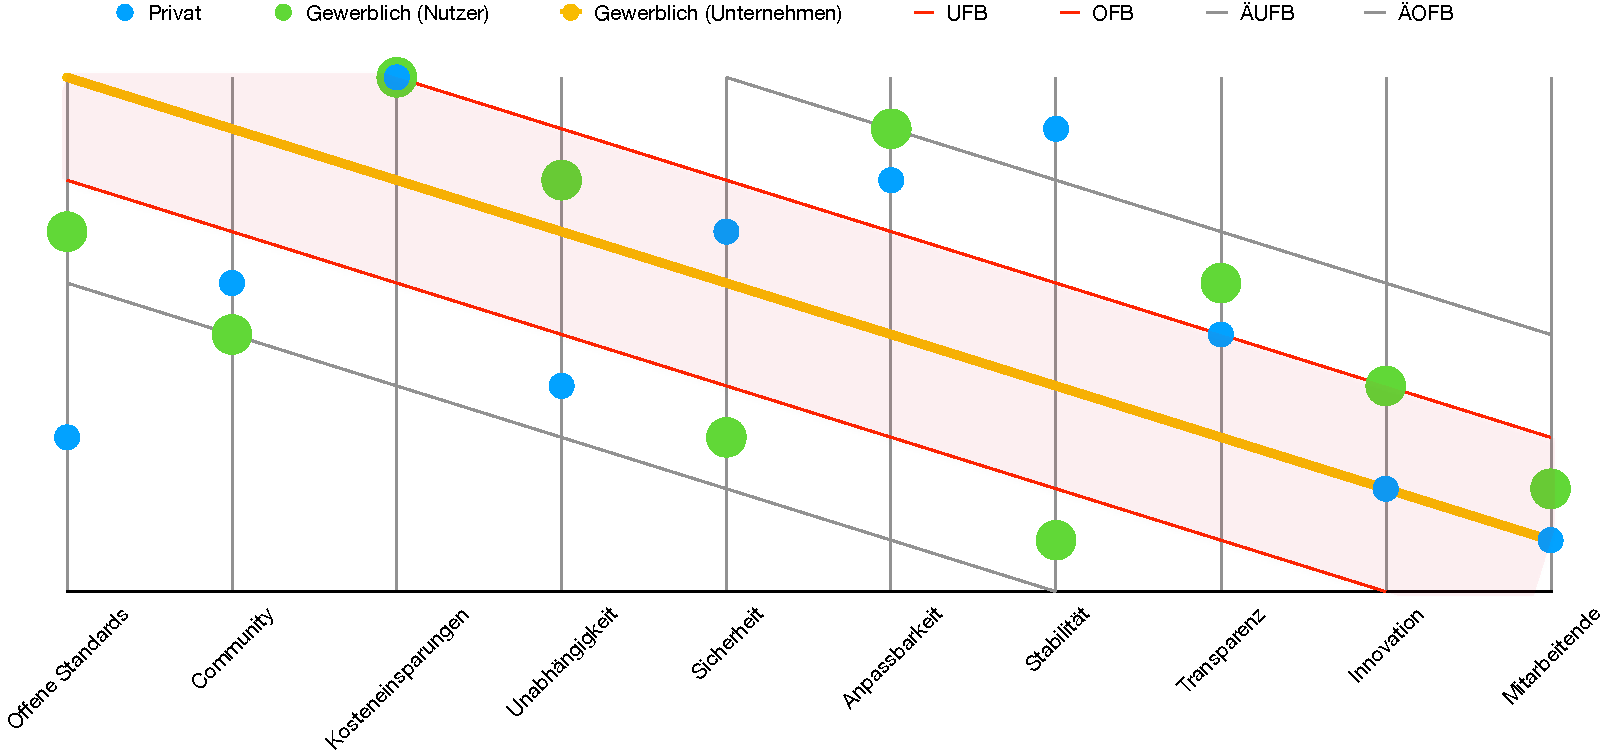
\includegraphics[width=\textwidth]{assets/results/commercialReasoning/usageReasonRanking}
                \caption{Ranking der Nutzungsgründe}
                \label{figure:usageRanking}
            \end{figure}
                
            \subsubsection{Aufbau des Diagramms}
                \paragraph{Kategorien}
                    Auf der x-Achse des Diagramms sind die Kategorien, welche der Schweizer Studie entnommen wurden, nach ihrer Wichtigkeit für Unternehmen von links nach rechts in absteigender Reihenfolge angeordnet.
                    
                \paragraph{Rankings}
                    Die y-Achse des Diagramms stellt die Wichtigkeit eines Aspekts für die Nutzung von \gls{oss} dar. Ein höherer Wert korrespondiert hierbei zu einer größeren Wichtigkeit.
                    
                \paragraph{innerer Fehlerbereich}
                    Der rot markierte Bereich stellt den inneren Toleranz- bzw. Fehlerbereich dar, welcher alle Werte mit einer Abweichung von dem Ranking der Unternehmen von maximal zwei einschließt. Sämtliche Datenpunkte, die sich in diesem Bereich befinden werden im folgenden als \"richtig\" angesehen, da ihre Abweichung von dem Zielwert nur gering ist.
                    
                \paragraph{äußerer Fehlerbereich}
                    Der Bereich zwischen den roten und grauen Linien wird im folgenden als äußerer Toleranz- bzw. Fehlerbereich genannt. Er beinhaltet alle Werte, dessen absolute Abweichung von dem Ranking der Unternehmen mehr als zwei und maximal vier entspricht.
                    
                \paragraph{Datenpunkte}
                    Das Diagramm beinhaltet drei verschiedene Werte für jede der Kategorien, wobei die Größe der Punkte keinerlei Bedeutung hat und lediglich dazu dient überlappende Punkte sichtbar zu machen. Im folgenden bezeichnen Datenpunkte ausschließlich die Werte, welche im Graphen grün eingezeichnet sind. Die Farben sind wie folgt zugeordnet:\\
                    \begin{table}[H]
                        \centering
                        \bgroup
                        \def\arraystretch{1.5}
                        \begin{tabular}{ r | l }
                            \emph{Blau} & private Nutzung aus Sicht der Endanwender\\
                            \emph{Grün} & gewerbliche Nutzung aus Sicht der Endanwender\\
                            \emph{Gelb} & tatsächliche gewerbliche Nutzungsgründe
                        \end{tabular}
                        \egroup
                    \end{table}
                    
                    Die Quellen der einzelnen Datensätze sind im Folgenden erläutert:
                    \subparagraph{private Nutzung} Wie Eingangs erwähnt wurde das Freifeld in der Umfrage nach Tabelle \ref{table:categories} gegliedert und diese anschließend den Kategorien der Studie zugeordnet. Diese Zuordnung ist in Tabelle \ref{table:privateToCommercialCategories} einzusehen.
                    
                    \subparagraph{Sicht der Nutzer auf Unternehmen} Die Antworten der Multiple-Choice Frage bezüglich des Rankings wurden kumuliert und darauf basierend ein Ranking erstellt.
                    
                    \subparagraph{gewerbliche Nutzung} Das Ranking für die gewerbliche Nutzung wurden Figur 8 auf Seite 16 der Schweizer Studie\cite{oss:studie} direkt entnommen.
            
            \subsubsection{Auswertung des Diagramms}
                \paragraph{Sicht der Nutzer auf Unternehmen}
                    Abbildung \ref{figure:usageRanking} kann man entnehmen, dass sich $40\%$ der Datenpunkte im inneren Fehlerbereich befinden ({\scriptsize Kosteneinsparungen, Unabhängigkeit, Innovation, Mitarbeitende}) und somit als richtig anzusehen sind. Komplementär dazu befinden sich $60\%$ der Datenpunkte im äußeren Fehlerbereich und \emph{keine} Datenpunkte außerhalb der Fehlerbereiche.\\
                    Dabei ist zu beachten, dass $20\%$ der Kategorien oberhalb ({\scriptsize Anpassbarkeit, Transparenz}) und $40\%$ unterhalb ({\scriptsize Offene Standards, Community, Sicherheit, Stabilität}) des inneren Toleranzbereichs liegen.
                    
                \paragraph{Abweichung von privaten Gründen}
                    Des weiteren ist auffällig, dass $60\%$ der Werte innerhalb des Toleranzbereichs\footnote{Der Toleranzbereich um die privaten Gründe ist im Diagramm nicht verzeichnet, hat aber die gleiche Toleranz wie der der gewerblichen Gründe und lässt sich daher nachmessen.} von den privaten Gründen liegen, wovon sich die Hälfte der Datenpunkte in dem inneren Fehlerbereich befindet.
                               
            \subsubsection{Interpretation der Daten}
                \paragraph{Abweichung von der Realität}
                    Betrachtet man den äußeren Toleranzbereich, so liegen die Nutzer mit ihrer Einschätzung grob richtig. Schaut man nun allerdings auf den inneren Fehlerbereich, so liegen sie nur noch mit $40\%$ der Kategorien mit ihrem Ranking in der unmittelbaren Nähe der Schweizer Unternehmen. Dies lässt darauf schließen, dass die allgemeine Ansicht welche Aspekte für Unternehmen von Bedeutung sind vorhanden, jedoch nicht stark ausgeprägt sind.\\
                    Des Weiteren ist auffällig, dass die Aspekte \emph{Offene Standards} und \emph{Stabilität} welche sich in Relation zu den privaten Gründen in die richtige Richtung orientieren beide zu schwach eingeschätzt wurden. % TODO Folgerung daraus? Wieso zu schwach?
                    
                \paragraph{Projektion privater Gründe}
                    Schaut man sich die Werte ausserhalb des inneren Fehlerbereichs an, so fällt auf, dass $50 \%$ der Punkte ({\scriptsize Community, Anpassbarkeit, Transparenz}) eine sehr geringe Distanz zu den privaten Gründen haben. Daraus lässt sich ableiten, dass die Nutzer möglicherweise ihre privaten Gründe auf Unternehmen projizieren.\\
                    Betrachtet man ebenfalls die Werte innerhalb des Toleranzbereichs, so findet man weitere Beispiele, welche diese These ({\scriptsize Kosteneinsparungen, Innovation, Mitarbeitende}) unterstreichen. Es lässt sich anhand der vorliegenden Daten allerdings nicht zweifelsfrei beweisen, dass die Punkte lediglich aufgrund der Projektion und nicht aufgrund des Wissens der Nutzer in dem inneren Fehlerbereich liegen.\\
                    Nimmt man alle Datenpunkte die eine maximale Abweichung von zwei zu den privaten Nutzungsgründen haben und geht davon aus, dass diese ihre aktuelle Position aufgrund der Projektion haben, so bleibt lediglich ein Punkt in dem inneren Toleranzbereich übrig. Dies ist der Aspekt der \emph{Unabhängigkeit}, welcher eindeutig von den Nutzern richtig in den inneren Toleranzbereich eingeordnet wurde.
    
        \subsection{Demographische Differenzen}
            Da es selten der Fall ist, dass Wissen in der Gesellschaft homogen verteilt ist, enthielt die Umfrage sowohl ein Frage zur Selbsteinschätzung der Computerkenntnisse als auch eine zur aktuellen Tätigkeit, um darauf basierend Verschiebungen in der Wissensverbreitung zu untersuchen.
            
            \subsubsection{Selbsteinschätzung}
                % TODO reference zu kritik: Nur daten, wenn oss genutzt
                Um zu ermitteln, ob es Differenzen bei verschiedenen Selbsteinschätzungen gibt, wurde die Korrektheit der Angabe, ob eine Software open source ist wie in Abschnitt \ref{section:knowledge_oss} nach Kategorie gruppiert ausgewertet. Dabei wurde aber die Antworten der Nutzer mit einer Selbsteinschätzung von eins bis vier (im Folgenden als Gruppe 1-4 bezeichnet) und die der Nutzer mit fünf oder sechs (im Folgenden als Gruppe 5-6 bezeichnet) getrennt zusammengefasst und in Abbildung \ref{figure:knowledge_by_category_self_assessment} dargestellt, um diese vergleichen zu können.
                
                \paragraph{Signifikanz}
                    Um die Signifikanz der Differenzen beurteilen zu können wurde ein Signifikanztest der Abweichung der Ergebnisse der Gruppe 5-6 zu den Ergebnissen der Gruppe 1-4 durchgeführt und in Tabelle \ref{table:knowledge_by_category_sigma_self_assessment} zusammengefasst.
                    
                    \subparagraph{Beschreibung der Tabelle}
                        Die Spalte \emph{1-4} gibt an, wie viel Prozent der Gruppe 1-4 korrekt \gls{oss} erkannt haben. Die Spalten \emph{5-6} und \emph{$\sum$5-6} geben an, wie viele Antworten der Gruppe 5-6 korrekt beziehungsweise insgesamt abgegeben wurden. Die restlichen Spalten sind wie in Abschnitt \ref{section:knowledge_analysis} zu verstehen.
                        
                    \subparagraph{Auswertung}
                        Die Signifikanz der Abweichung ist in fast allen Kategorien sowie in der Gesamtauswertung hoch. Besonders extrem sind die Unterschiede in den Kategorien Browser und Betriebsysteme. Es ist aber zu beachten, dass die Gruppe 5-6 in der Kategorie Browser und die Gruppe 1-4 in der Kategorie Betriebsysteme lediglich 50\% erreicht haben und damit nach der Auswertung in Abschnitt \ref{section:knowledge_analysis} kein Wissen vorhanden ist. Das bedeutet, dass die zwei Differenz zwei verschiedene Ursachen haben: Einmal liegt es am falschen Wissen der Gruppe 1-4 und einmal an der richtigen Wissen der Gruppe 1-5.
                        
                        Insgesamt ist die Gruppe 5-6 besser als die Gruppe 1-4, wenn es um das Wissen über \gls{oss} geht. Diese Ergebnis deckt sich mit den Erwartungen aus Abschnitt \ref{section:fragestellung}.
                    
                \begin{figure}
                    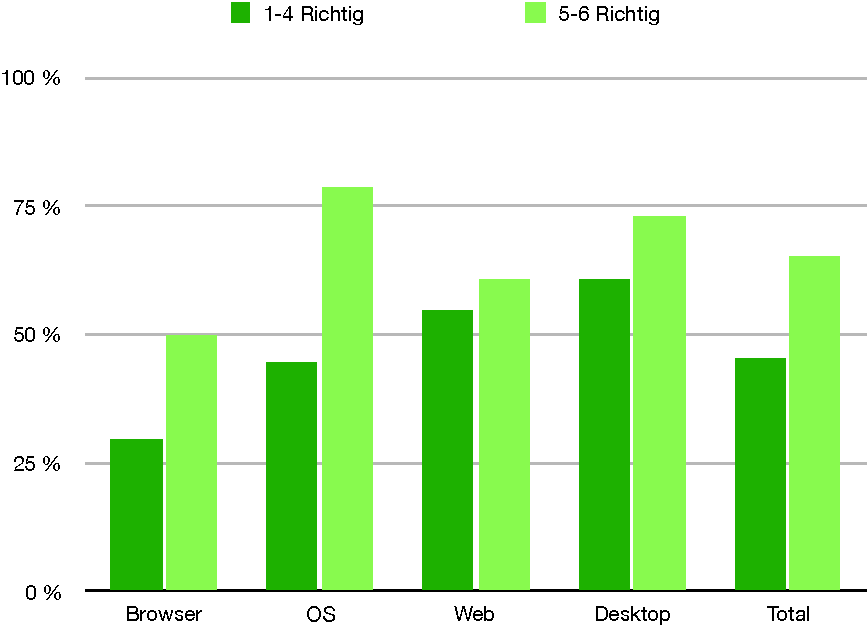
\includegraphics[width=\textwidth]{assets/results/openSourceJudging/openSourceJudgingDetailedOSSOnlyByKnowledge.pdf}
                    \caption{Wissen über \gls{oss} nach Selbsteinschätzung}
                    \label{figure:knowledge_by_category_self_assessment}
                \end{figure}
                
                \begin{table}
                    \centering
                    \begin{tabular}{rcccccc}
                        Kategorie & 1-4 & 5-6 & $\sum$ 5-6 & $2\sigma$-Umgebung & $3\sigma$-Umgebung & Signifikanz \\\hline\hline
                        Browser & $29.47\%$ & $75$ & $151$ & \tiny [ 33.3003 ; 55.7102 ] & \tiny [ 27.6978 ; 61.3127 ] & Hoch\\
                        OS & $44.74\%$ & $66$ & $84$ & \tiny  [ 28.4647 ; 46.6932 ]  &  \tiny  [ 23.9076 ; 51.2503 ]  & Hoch\\
                        Web & $54.55\%$ & $70$ & $115$ & \tiny [ 52.0479 ; 73.4067 ] &  \tiny  [ 46.7082 ; 78.7464 ]  &  Signifikant\\
                        Desktop & $60.66\%$ & $158$ & $217$ & \tiny  [ 117.2304 ; 146.0155 ]  & \tiny  [ 110.0342 ; 153.2117 ]  & Hoch\\\hline
                        Gesamt & $45.38\%$ & $369$ & $567$ & \tiny [ 233.6207 ; 281.0409 ] & \tiny  [ 221.7656 ; 292.8959 ]  & Hoch
                    \end{tabular}
                    \caption{Signifikanz der Abweichung nach Selbsteinschätzung}
                    \label{table:knowledge_by_category_sigma_self_assessment}
                \end{table}
            
            \subsubsection{Tätigkeit}
                Der zweite Aspekt, der hier zur Auswertung der demographischen Differenzen behandelt wird, ist die aktuelle Tätigkeit und damit indirekt, wenn auch nicht eindeutig, verbunden das Alter der Befragten. Zur Auswertung wurden die Tätigkeiten in die Gruppen `Schüler`, `Student` und `Arbeitstätig` unterteilt. Wie auch bei der Selbsteinschätzung wurden diese Gruppen verwendet, um das Wissen über \gls{oss} zu vergleichen. Wie in der graphischen Darstellung in Abbildung \ref{figure:knowledge_by_occupation} zu sehen hat keine der Gruppen in mehreren Kategorien gleichartig auffällige Abweichung und auch in der Gesamtauswertung sind keine Auffälligkeiten zu erkennen. Die aktuelle Tätigkeit oder das Alter scheint nur begrenzt Auswirkungen auf das Wissen über \gls{oss} zu haben.
            
            \begin{figure}
                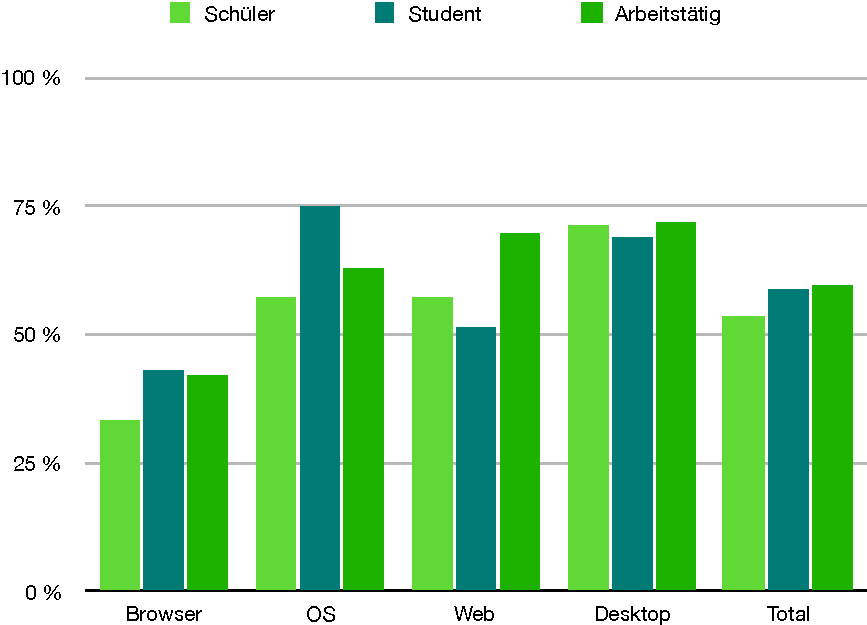
\includegraphics[width=\textwidth]{assets/results/openSourceJudging/openSourceJudgingDetailedOSSOnlyByOccupation.pdf}
                \caption{Wissen über \gls{oss} nach Tätigkeit}
                \label{figure:knowledge_by_occupation}
            \end{figure}
            
    
    
    \clearpage
    \section{Zusammenfassung}
        \subsection{Selbstreflexion}\label{section:selbstreflexion}
            Im Folgenden wird kritisch auf das Vorgehen in dieser Arbeit eingegangen und mögliche Methoden zur Optimierung der Ergebnisse dargelegt.
            \paragraph{Wann ist eine Software Open Source?}
                In der Umfrage wurde lediglich erwähnt, dass eine Software im Sinne der Umfrage auch als Open Source gilt, wenn sie \gls{oss} beinhaltet. Wie bereits Eingangs beschrieben, werden genutzte Programmiersprachen oder Datenbanken nicht als signifikante Open Source Komponente betrachtet. Dies wurde aus dem Fragebogen nicht ersichtlich und man hätte für bessere Umfrageergebnisse genauer spezifizieren müssen, dass eine Anwendung als Open Source gilt, wenn sie selbst quelloffen ist aber auch dann, wenn ihre Funktionalität durch die Entfernung von Open Source Komponenten signifikant eingeschränkt wäre.
                
            \paragraph{Enthaltung}
                Da der Fragebogen bei der Anwendungsmatrix lediglich die Optionen \emph{Ja} und \emph{Nein} beinhaltete besteht die Möglichkeit, dass die Befragten die Felder auf ihrem Standardwert ({\scriptsize Nein}) belassen haben, wenn sie sich unsicher waren. Dies hätte man umgehen können, indem man eine dritte Option für das Feld einfügt, welche Enthaltung repräsentiert. Um der potentiellen Verfälschung der Ergebnisse entgegenzuwirken wurden in dieser Arbeit lediglich die Datenpunkte der Nutzer in Betracht gezogen, die auch angegeben haben die Anwendung zu verwenden.
                
            \paragraph{Kategorisierung}
                Für die privaten Nutzungsgründe gab es in der Umfrage ein Freifeld. Für den Vergleich in Abschnitt \ref{section:usageReasons} war es nötig die abgegebenen Stimmen in die Kategorien der Studie bzgl. der Unternehmen einzuordnen, was aufgrund der grundverschiedenen Anwendungszwecke dazu geführt hat, dass in dem Diagramm einige Stimmen der privaten Nutzungsgründe aufgrund der fehlenden Übereinstimmung mit den kommerziellen Kategorien nicht repräsentiert sind.
                
            \paragraph{Kulturelle Differenzen}
                Es ist auf Basis der genutzten Verbreitungsmedien zu vermuten, dass die Datensätze überwiegend Stimmen aus Deutschland enthalten. Die Vergleichsstudien stammen aus Österreich\cite{demographicDistributionKnowledge} und der Schweiz\cite{oss:studie}. Dabei ist nicht auszuschließen, dass aufgrund diverser wirtschaftlicher, politischer, ideologischer und kulturelle Gründe die demographische Verteilung und IT-Kenntnisse sowie Nutzungsgründen von denen in Deutschland abweichen. Dies lässt sich auf Basis der vorliegenden Daten nicht ausschließen, aber es ist aufgrund der geografischen Nähe und nahezu identischen Sprache der drei zuvor genannten Ländern wahrscheinlich, dass die Abweichung nur gering ausfällt.
                
            \paragraph{Spiele}
                Die Anwendungsmatrix in der Umfrage beinhaltete eine Kategorie zu Computerspielen. Diese Kategorie beinhaltete aufgrund eines Fehlers auf Seiten der Autoren ausschließlich Spiele, welche nicht Open Source sind und nur unsignifikante Mengen von Open Source Software für die kritische Funktionalität verwenden. Dies führte dazu, dass alle Datenpunkte aus dieser Kategorie für die Auswertung im Rahmen der drei in dieser Arbeit betrachteten Hauptaspekte nicht verwendbar waren. Aus dem Datensatz lässt sich lediglich schließen, dass $88.6\%$ der Leute, welche die Spiele nutzen, diese korrekt als Closed-Source einschätzten.
            
        \subsection{Fazit}
            % TODO
        
    
    \clearpage
    \section{Eidesstattliche Erklärung}
        Hiermit erklären wir, dass wir die vorliegende Hausarbeit selbstständig verfasst und keine anderen als die angegebenen Hilfsmittel benutzt haben.\\
        Die Stellen der Hausarbeit, die andere Quellen im Wortlaut oder dem Sinn nach entnommen wurden, sind durch Angabe der Herkunft kenntlich gemacht. Dies gilt auch für Zeichnungen, Skizzen, bildliche Darstellungen sowie für Quellen aus dem Internet.
        
        
        \begin{figure}[H]
            \centering
            \begin{minipage}{.5\textwidth}
                \centering
                
\includegraphics[width=\textwidth]{assets/signature_tilb.png}
                Til Blechschmidt
            \end{minipage}%
            \begin{minipage}{.5\textwidth}
                \centering
                
\includegraphics[width=\textwidth]{assets/signature_noahp.png}
                Noah Peeters
            \end{minipage}
        \end{figure}
        \clearpage
    
    \clearpage
    \section{Appendix}
        \printglossary[type=\acronymtype]
        \printglossary
        
        \clearpage
        \nocite{*}
        \bibliographystyle{unsrt}
        \bibliography{Bibliography}
        
        \clearpage
        
        \subsection{Abschnitte}
            \begin{tabular}{rl}
              Abschnitt & Autor \\
              \hline
              Bla & N. Peeters\\
              Bla & T. Blechschmidt
            \end{tabular}
        
%        \subsection{Umfrage}
%            \paragraph{Ergebnisse}
%                Die Ergebnisse der Umfrage liegen als CSV-Datei bei und sind auch in dieses PDF eingebunden: \attachfile{assets/Open Source.csv}
%            \paragraph{Fragebogen}
%                Auf den nächsten vier Seiten befindet sich eine PDF-Version des Fragebogens, wie er Online verbreitet wurde.
%                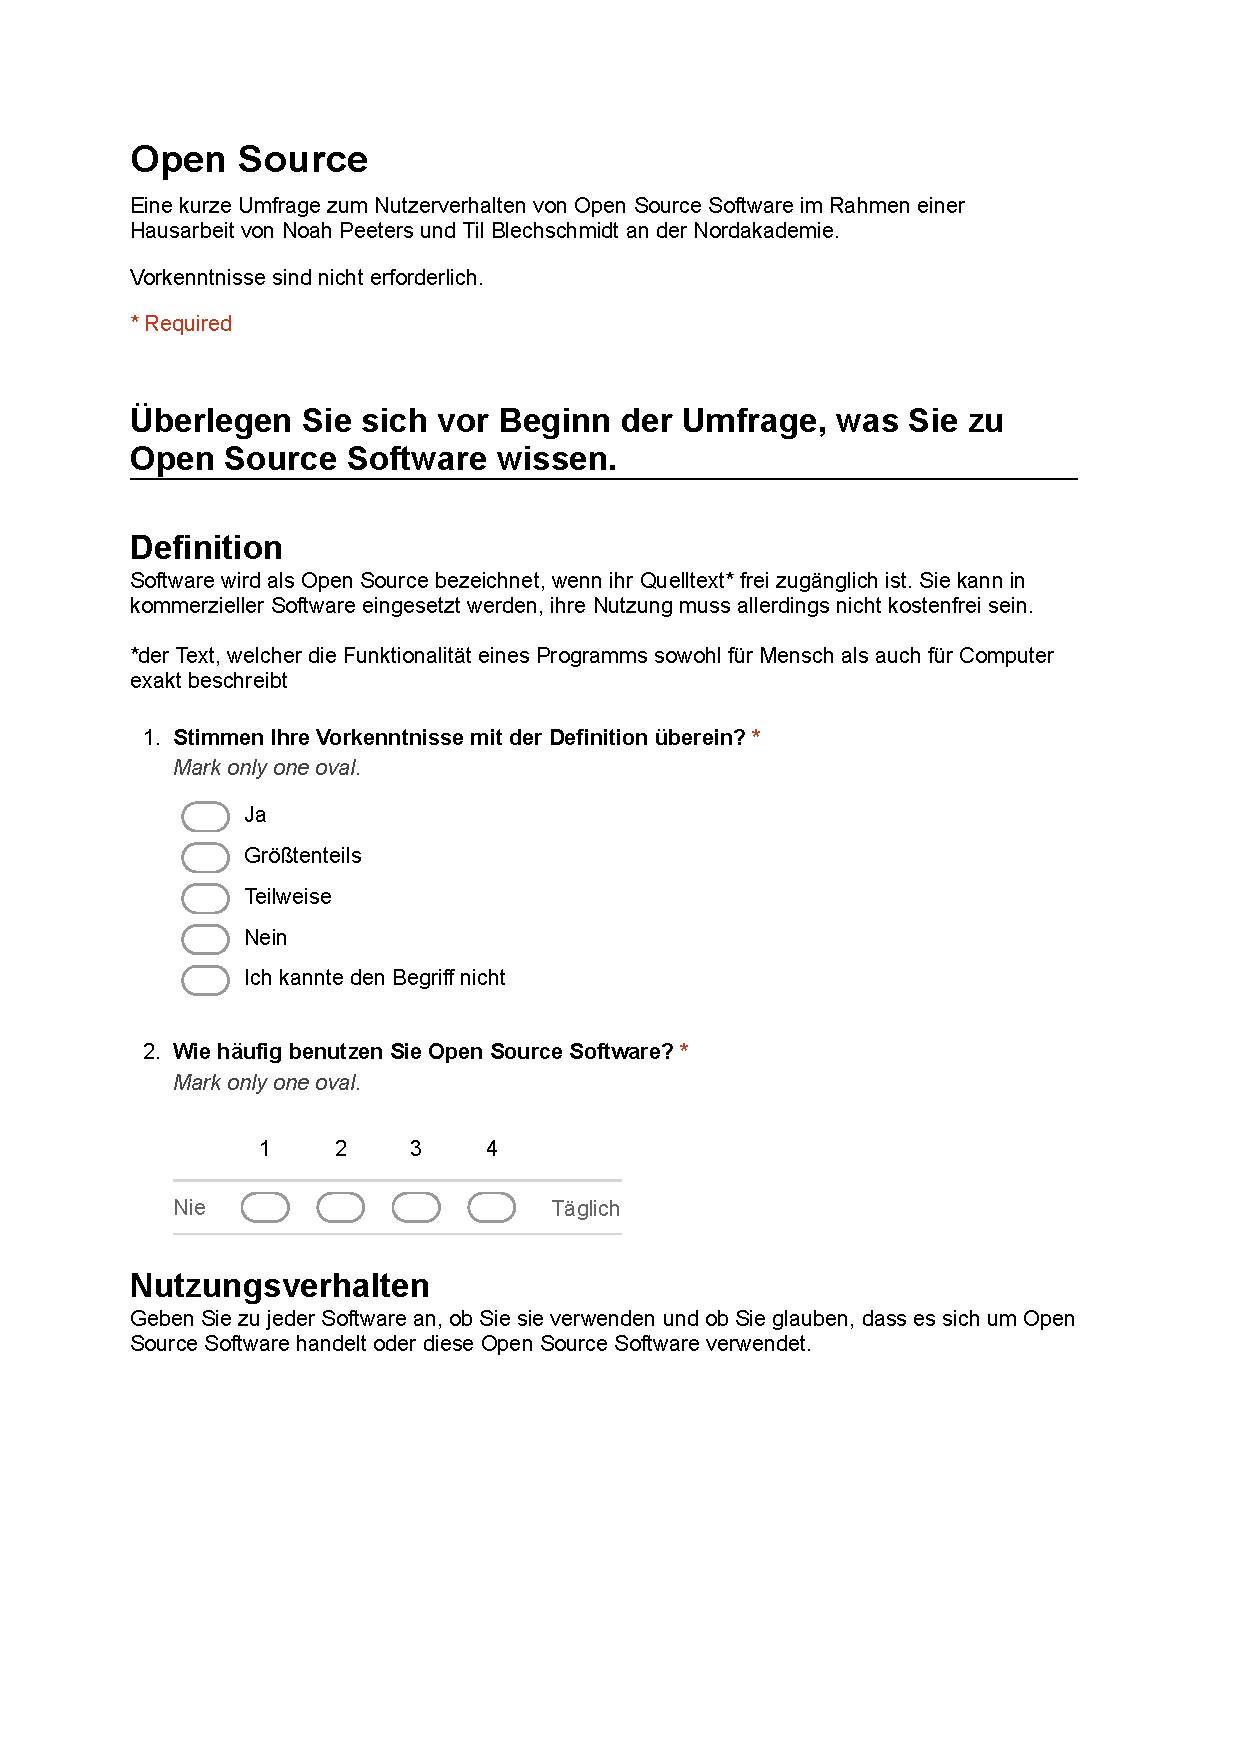
\includepdf[pages={-}]{assets/Umfrage.pdf}

\end{document}
